\section{Уравнения механики деформируемого твёрдого тела}
\subsection{Уравнения движения и реологические соотношения}
Для математического моделирования волновых процессов в деформируемом твёрдом
теле используется система динамических уравнений \cite{novatsky,sedov} в виде
\begin{eqnarray}
\label{rheology_equations}
\rho\dot{v}_i=\nabla_j\sigma_{ij}+f_i & \textrm{(уравнения движения)}\nonumber\\
\dot{\sigma}_{ij}=q_{ijkl}\dot{\varepsilon}_{kl}+F_{ij} & \textrm{(реологические
соотношения).}
\end{eqnarray}

Здесь $\rho$ – плотность среды, $v_i$ – компоненты скорости смещения,
$\sigma_{ij}$, $\varepsilon_{ij}$ -- компоненты тензоров напряжений и деформаций,
$\nabla_j$ – производная по $j$-й координате, $f_i$ – массовые
силы, действующие на единицу объёма, $F_{ij}$ -- силы, обусловленные вязкостью, $q_{ijkl}$ -- 
тензор упругих постоянных.

В случае малых деформаций тензор скоростей деформаций $e_{ij}=\dot{\varepsilon}_{ij}$ 
выражается через компоненты скорости смещения линейным образом:
\begin{equation}
e_{ij}=\frac{1}{2}(\nabla_j v_i+\nabla_i v_j).
\end{equation}

Вид компонент тензора 4-го порядка $q_{ijkl}$ определяется реологией среды. Для 
невязкого изотропного линейно-упругого материала
\begin{eqnarray}
\label{tensor_qijkl}
q_{ijkl}=\lambda\delta_{ij}\delta_{kl}+\mu(\delta_{ik}\delta_{jl}+\delta_{il}
\delta_{jk}) & \textrm {(изотропия)} \nonumber\\
F_{ij}=0 & \textrm {(отсутствует вязкость).}
\end{eqnarray}
В этом соотношении, которое обобщает закон Гука, $\lambda$ и $\mu$ -- параметры
Ляме, $\delta_{ij}$ -- символ Кронекера.

Для замыкания системы уравнений \ref{rheology_equations} её необходимо дополнить
уравнением состояния, определяющим зависимость плотности от напряжений:
например, $$\rho=const$$ или
$$\rho=\rho_0e^{\frac{p}{K}},$$
где $p=-\frac{1}{3}\sum\sigma_{kk}$ -- давление, $K=\lambda+\frac{2}{3}\mu$ --
коэффициент всестороннего сжатия.

\subsection{Модель пластического течения}
Существует множество феноменологических моделей пластической реологии сплошной среды.
Основная идея многих из них \cite{resler,kukudganov} -- существование критерия текучести $f(\sigma_{ij})$, определяющего переход между упругим $f(\sigma_{ij})<0$ и пластическим $f(\sigma_{ij})=0$ поведением материала. Компоненты $\sigma_{ij}$ не могут выйти за пределы поверхности в пространстве напряжений, определяемой этим критерием, случай $f(\sigma_{ij})>0$ полагается невозможным.
 
Таким образом, идеальнопластическим материалом, или материалом без упрочнения, можно назвать среду с постоянной функцией $f(\sigma_{ij})$, а материалом с упрочнением -- тот, у которого поверхность текучести изменяется в процессе деформации. Выделяют два основных вида упрочнения:
\begin{itemize}
\item Изотропное -- поверхность текучести расширяется симметрично относительно начала координат
\item Кинематическое -- поверхность текучести смещается без изменения формы
\end{itemize} 

Для металлов установлено, что пластическая деформация обусловлена взаимным смещением кристаллических плоскостей и не изменяет объёма материала. Поэтому гидростатическое сжатие $$\sigma = \frac{\sigma_{ii}}{3}$$ не приводит к пластическим деформациям, и переход к пластике определяется только сдвиговыми напряжениями, то есть девиатором тензора напряжений: $$s_{ij} = \sigma_{ij} - \sigma\delta_{ij}$$ 
\subsubsection{Критерий текучести Мизеса}
Одним из широко используемых критериев является получаемая из инвариантов $\sigma_{ij}$ функция
\begin{eqnarray}
\label{mizes}
f(\sigma_{ij}) = \frac{1}{2}s_{ij}s_{ji} - k^2_F
\end{eqnarray}

Получаемая поверхность текучести -- круговой цилиндр радиуса $k_F\sqrt{2}$ с осью $\sigma_1 = \sigma_2 = \sigma_3$ в пространстве главных напряжений. На рис.\ref{pic:mizes} приведено его сечение плоскостью $\sigma_3 = 0$, а также сечение другой поверхности, получаемой из близкого к мизесовскому критерия Треска.

\begin{figure}
\center{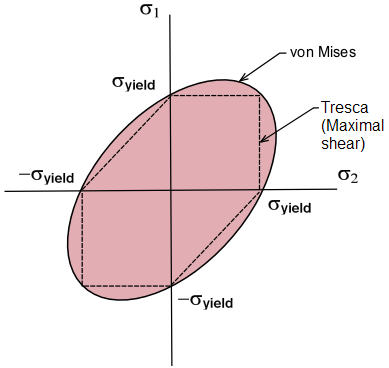
\includegraphics[width=\textwidth]{png/mizesa_criteriy.png}}
\caption{Критерий текучести.}
\label{pic:mizes}
\end{figure}

Для полимеров же величина предела текучести при сжатии и растяжении часто бывает различна. Поэтому в критерий текучести включаются слагаемые, зависящие от гидростатического давления, и поверхность текучести из цилиндрической переходит в коническую или близкую к ней.

В программном комплексе для случая трёх измерений была реализована модель идеального пластического течения без упрочнения, которая в случае одноосного нагружения сводится к диаграмме $\varepsilon-\sigma$ на рис.\ref{pic:ideal_plastic}

\begin{figure}
\center{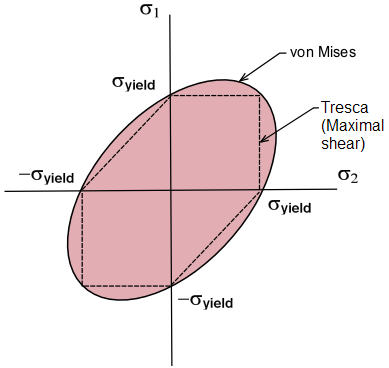
\includegraphics[width=\textwidth]{png/mizesa_criteriy.png}}
\caption{Идеальная упругопластика в случае одноосного нагружения.}
\label{pic:ideal_plastic}
\end{figure}

Для одномерного кода были испробованы модели с линейным упрочнением. В 1D такая модель сводится к кусочной зависимости модуля Юнга от напряжения (рис. \ref{pic:uprochnenie})

\begin{figure}
\center{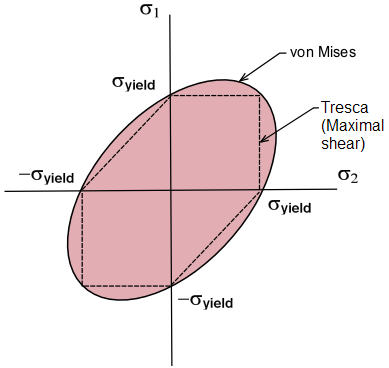
\includegraphics[width=\textwidth]{png/mizesa_criteriy.png}}
\caption{Упругопластика с линейным упрочнением.}
\label{pic:uprochnenie}
\end{figure}

